\let\negmedspace\undefined
\let\negthickspace\undefined
\documentclass[journal,12pt,twocolumn]{IEEEtran}
\usepackage{float}
\usepackage{circuitikz}
\usepackage{cite}
\usepackage{amsmath,amssymb,amsfonts,amsthm}
\usepackage{algorithmic}
\usepackage{graphicx}
\usepackage{textcomp}
\usepackage{xcolor}
\usepackage{txfonts}
\usepackage{listings}
\usepackage{amsmath}
\usepackage{enumitem}
\usepackage{mathtools}
\usepackage{gensymb}
\usepackage{comment}
\usepackage[breaklinks=true]{hyperref}
\usepackage{tkz-euclide} 
\usepackage{listings}
\usepackage{gvv}                                        
\def\inputGnumericTable{}                                 
\usepackage[latin1]{inputenc}                                
\usepackage{color}                                            
\usepackage{array}                                            
\usepackage{longtable}                                       
\usepackage{calc}  
\usepackage{caption}
\usepackage{multirow}                                         
\usepackage{hhline}                                           
\usepackage{ifthen}                                           
\usepackage{lscape}
\newtheorem{theorem}{Theorem}[section]
\newtheorem{problem}{Problem}
\newtheorem{proposition}{Proposition}[section]
\newtheorem{lemma}{Lemma}[section]
\newtheorem{corollary}[theorem]{Corollary}
\newtheorem{example}{Example}[section]
\newtheorem{definition}[problem]{Definition}
\newcommand{\BEQA}{\begin{eqnarray}}
\newcommand{\EEQA}{\end{eqnarray}}
\newcommand{\define}{\stackrel{\triangle}{=}}
\theoremstyle{remark}
\newtheorem{rem}{Remark}
\renewcommand\thesection{\arabic{section}}
\renewcommand\thesubsection{\thesection.\arabic{subsection}}
\renewcommand\thesubsubsection{\thesubsection.\arabic{subsubsection}}

\renewcommand\thesectiondis{\arabic{section}}
\renewcommand\thesubsectiondis{\thesectiondis.\arabic{subsection}}
\renewcommand\thesubsubsectiondis{\thesubsectiondis.\arabic{subsubsection}}
\lstset{
language=Python,
frame=single, 
breaklines=true,
columns=fullflexible
}
\numberwithin{equation}{subsection}
\renewcommand{\thesubsection}{\thesection.\arabic{subsection}}


\begin{document}

\bibliographystyle{IEEEtran}

\numberwithin{equation}{section}



\renewcommand{\thefigure}{\theproblem.\arabic{figure}}
\renewcommand{\thefigure}{\theproblem}




\vspace{3cm}

\title{Audio Filtering}

\author{EE23BTECH11009 - AROSHISH PRADHAN$^{*}$}

\maketitle

\tableofcontents

\renewcommand{\thefigure}{\theenumi}
\renewcommand{\thetable}{\theenumi}
\bigskip

\begin{abstract}
This manual attempts digital signal processing of an audio file.
\end{abstract}

\section{Software Installation}
Run the following commands
\begin{lstlisting}
sudo apt-get update
sudo apt-get install libffi-dev libsndfile1 python3-scipy  python3-numpy python3-matplotlib 
sudo pip install cffi pysoundfile 
\end{lstlisting}
\section{Digital Filter}
\begin{enumerate}[label=\thesection.\arabic*
,ref=\thesection.\theenumi]
\item
\label{prob:input}
Download the sound file from  
\begin{lstlisting}
wget https://github.com/aroshishp/EE1205/blob/main/Audio_Filtering/codes/2.wav
\end{lstlisting}

\item
\label{prob:spectrogram}
You will find a spectrogram at \href{https://academo.org/demos/spectrum-analyzer}{\url{https://academo.org/demos/spectrum-analyzer}}. 

Upload the sound file that you downloaded in Problem \ref{prob:input} in the spectrogram  and play.  Observe the spectrogram. What do you find?
\\

\solution The purple areas of the spectrogram represent frequencies with low intensities (noise) while the red-yellow regions represent frequnecies with high intensities (voice). 

\begin{figure}[!h]
    \centering
    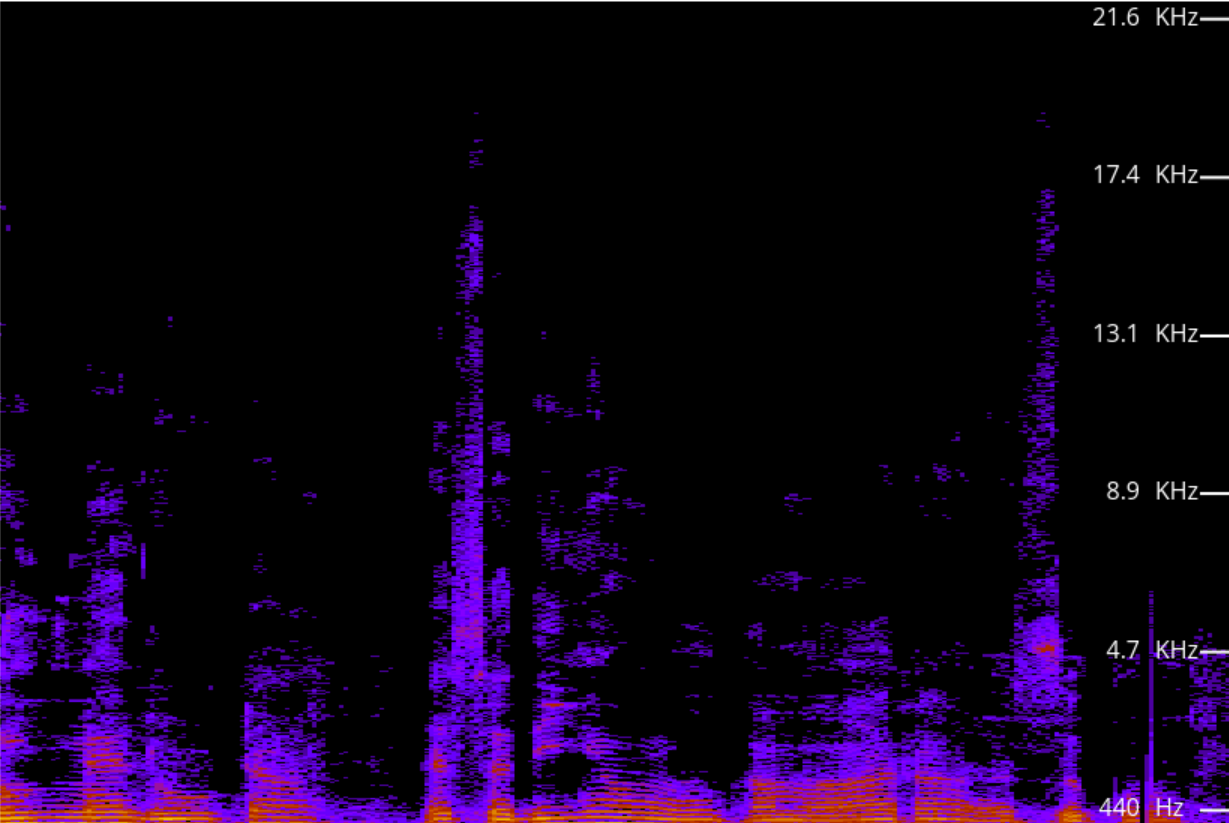
\includegraphics[width = \columnwidth]{figs/unfiltered.png}
    \caption{Spectrogram before filtering}
    \label{fig:2.2}
\end{figure}

\item
\label{prob:output}
Write the python code for removal of out of band noise and execute the code.
\\

\solution Noise in the audio is     filtered out using the following python code:
\begin{lstlisting}

import soundfile as sf
from scipy import signal

# Read .wav file
inpu_signal, fs = sf.read('2.wav')

# Order of the filter
order = 4

# Cutoff frequency 6kHz
cutoff_freq = 6000.0

# Digital frequency
Wn = 2 * cutoff_freq / fs

# b and a are numerator and denominator polynomials, respectively
b, a = signal.butter(order, Wn, 'low')

print(a)
print(b)

output_signal = signal.lfilter(b,a, input_signal)
# Write the output signal into a .wav file
sf.write('2_fil.wav', output_signal, fs)
\end{lstlisting} \label{py:filter}

\item
The output of the python script in Problem \ref{prob:output} is the audio file 2\_fil.wav. Play the file in the spectrogram in Problem \ref{prob:spectrogram}. What do you observe?
\\

\solution 
\begin{figure}[!h]
    \centering
    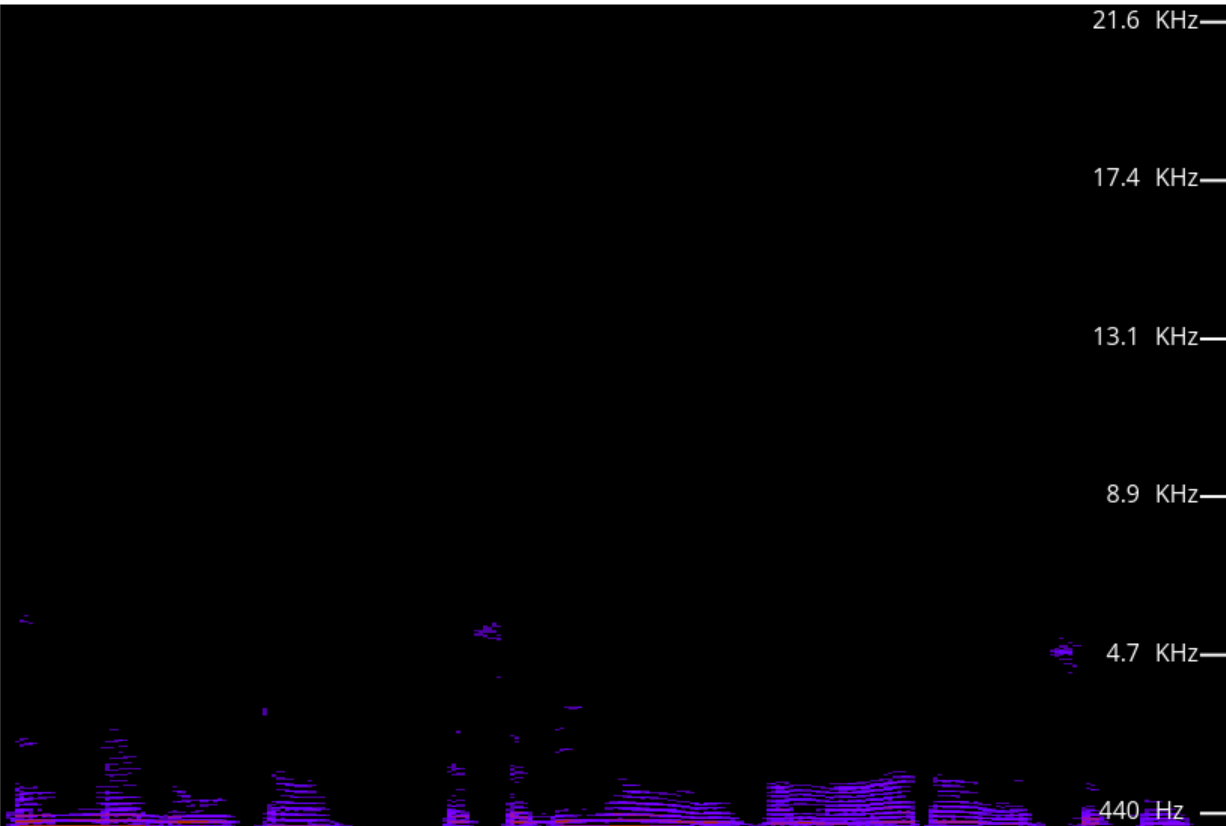
\includegraphics[width = \columnwidth]{figs/filtered.png}
    \caption{Spectrogram after filtering}
    \label{fig:2.3}
\end{figure}

The background noise (low intensities) is subdued in the audio.  Also,  the signal is blank for frequencies above 6 kHz.

\end{enumerate}

\section{Difference Equation}
\begin{enumerate}[label=\thesection.\arabic*,ref=\thesection.\theenumi]
\item Let
\begin{equation}
x(n) = \cbrak{\underset{\uparrow}{1},2,3,4,2,1}
\end{equation}
Sketch $x(n)$.\\

\solution The following code yields Fig. \ref{fig:x_n}.
\begin{lstlisting}
wget https://github.com/aroshishp/EE1205/blob/main/Audio_Filtering/codes/3.1.py
\end{lstlisting}
\begin{figure}[!h]
    \centering
    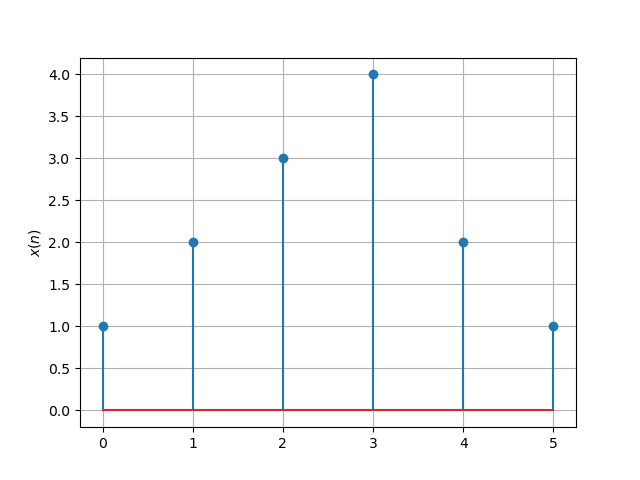
\includegraphics[width = \columnwidth]{figs/3.1.png}
    \caption{Digital Filter Input $x(n)$}
    \label{fig:x_n}
\end{figure}

\item Let
\begin{multline}
\label{eq:iir_filter}
y(n) + \frac{1}{2}y(n-1) = x(n) + x(n-2), 
\\
 y(n) = 0, n < 0
\end{multline}
Sketch $y(n)$.
\\
\solution The following codes yield Fig. \ref{fig:y_n}.
\begin{lstlisting}
wget https://github.com/aroshishp/EE1205/blob/main/Audio_Filtering/codes/3.2.c

wget https://github.com/aroshishp/EE1205/blob/main/Audio_Filtering/codes/3.2.py
\end{lstlisting}
\begin{figure}[!h]
\begin{center}
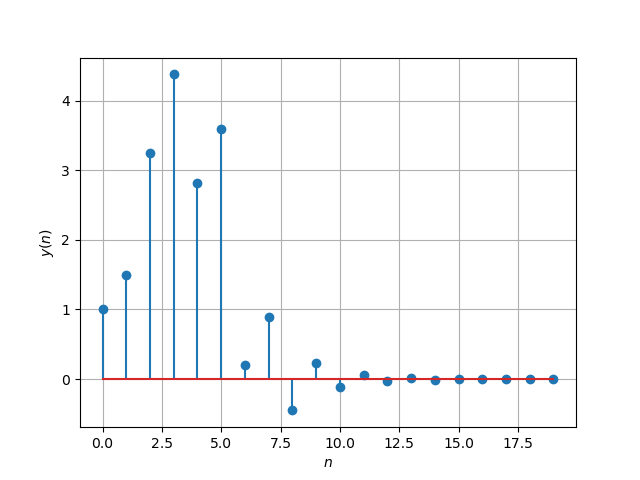
\includegraphics[width=\columnwidth]{figs/3.2.png}
\end{center}
\caption{Digital Filter Output $y(n)$}
\label{fig:y_n}	
\end{figure}

\end{enumerate}
\section{Z-transform}
\begin{enumerate}[label=\thesection.\arabic*]
\item The $Z$-transform of $x(n)$ is defined as
\begin{equation}
\label{eq:4.1}
X(z)={\mathcal {Z}}\{x(n)\}=\sum _{n=-\infty }^{\infty }x(n)z^{-n}
\end{equation}
%
Show that
\begin{equation}
\label{eq:4.2}
{\mathcal {Z}}\{x(n-1)\} = z^{-1}X(z)
\end{equation}
and find
\begin{equation}
	{\mathcal {Z}}\{x(n-k)\} 
\end{equation}
\solution From \eqref{eq:4.1},
\begin{align}
{\mathcal {Z}}\{x(n-1)\} &=\sum _{n=-\infty }^{\infty }x(n-1)z^{-n}\\
n &\longrightarrow n+1\\ \nonumber
&=\sum _{n=-\infty }^{\infty }x(n)z^{-n-1} \\
&= z^{-1}\sum _{n=-\infty }^{\infty }x(n)z^{-n}\\
&= z^{-1}X(z)
\end{align}
resulting in \eqref{eq:4.2}. Similarly, it can be shown that
%
\begin{align}
{\mathcal {Z}}\{x(n-k)\} &=\sum _{n=-\infty }^{\infty }x(n-k)z^{-n}\\
n &\longrightarrow n+k \nonumber\\
&=\sum _{n=-\infty }^{\infty }x(n)z^{-n-k} \\
&= z^{-k}\sum _{n=-\infty }^{\infty }x(n)z^{-n}\\
&= z^{-k}X(z) \label{eq:4.11}
\end{align}

\item Find
%
\begin{equation}
H(z) = \frac{Y(z)}{X(z)}
\end{equation}
%
from  \eqref{eq:iir_filter} assuming that the $Z$-transform is a linear operation.
\\
\solution Using \eqref{eq:4.11} in \eqref{eq:iir_filter},
\begin{align}
Y(z) + \frac{1}{2}z^{-1}Y(z) &= X(z)+z^{-2}X(z)
\\
\implies \frac{Y(z)}{X(z)} &= \frac{1 + z^{-2}}{1 + \frac{1}{2}z^{-1}}
\label{eq:freq_resp}
\end{align}
%
\item Find the Z transform of 
\begin{equation}
\delta(n)
=
\begin{cases}
1 & n = 0
\\
0 & \text{otherwise}
\end{cases}
\end{equation}
and show that the $Z$-transform of
\begin{equation}
\label{eq:unit_step}
u(n)
=
\begin{cases}
1 & n \ge 0
\\
0 & \text{otherwise}
\end{cases}
\end{equation}
is
\begin{equation}
U(z) = \frac{1}{1-z^{-1}}, \quad \abs{z} > 1
\end{equation}
\solution
\begin{align}
{\mathcal{Z}}\{\delta(n)\} &= \sum_{n=-\infty}^{\infty}\delta(n)z^{-n}\\
&= \delta(0)z^{-0}\\
&= 1
\end{align}
and from \eqref{eq:unit_step},
\begin{align}
U(z) &= \sum _{n= 0}^{\infty}z^{-n}
\\
&=\frac{1}{1-z^{-1}}, \quad \abs{z} > 1
\end{align}
using the formula for the sum of an infinite geometric progression.
%
\item Show that 
\begin{equation}
\label{eq:anun}
a^nu(n) \system \frac{1}{1-az^{-1}} \quad \abs{z} > \abs{a}
\end{equation}
%
\solution
\begin{align}
    {\mathcal{Z}}\{a^nu(n)\} &= \sum_{n=-\infty}^{\infty}a^nu(n)z^{-n}\\
    &= \sum_{n=0}^{\infty}(az^{-1})^n\\
    &= \frac{1}{1 - az^{-1}} \quad \abs{z} > \abs{a}
\end{align}
using the formula for the sum of an infinite geometric progression.
\item 
Let
\begin{equation}
H\brak{e^{j \omega}} = H\brak{z = e^{j \omega}}.
\end{equation}
Plot $\abs{H\brak{e^{j \omega}}}$.  Comment.  $H(e^{j \omega})$ is
known as the {\em Discrete Time Fourier Transform} (DTFT) of $h(n)$.
\\
\solution The following codes plot Fig. \ref{fig:dtft}.
\begin{lstlisting}
wget https://github.com/aroshishp/EE1205/blob/main/Audio_Filtering/codes/4.5.c

wget https://github.com/aroshishp/EE1205/blob/main/Audio_Filtering/codes/4.5.py
\end{lstlisting}
\begin{figure}[!h]
\centering
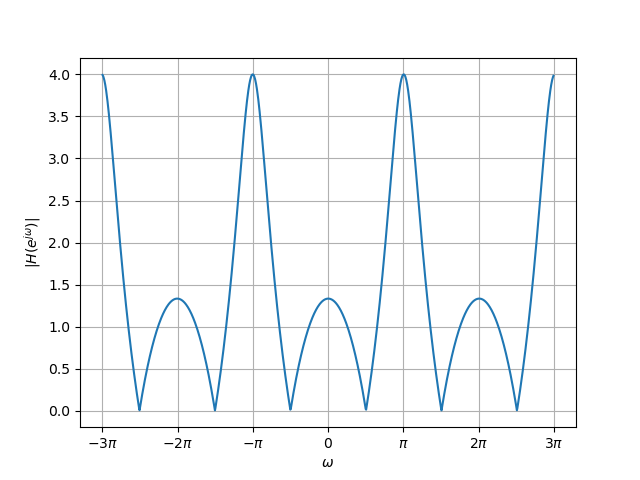
\includegraphics[width=\columnwidth]{figs/4.5.png}
\caption{Plot of $\abs{H\brak{e^{j\omega}}}$}
\label{fig:dtft}
\end{figure}

Substituting $z = e^{j \omega}$ in \eqref{eq:freq_resp},
\begin{align}
    \abs{H(e^{j\omega})} &= \abs{\frac{1 + e^{-2j\omega}}{1 + \frac{1}{2}e^{-j\omega}}}\\
    &= \frac{\sqrt{\brak{1 + \cos{2\omega}}^2 + \brak{\sin{2\omega}}^2}}{\sqrt{\brak{1 + \frac{\cos{\omega}}{2}}^2 + \brak{\frac{\sin{\omega}}{2}}^2}}\\
    &= \frac{4|\cos{\omega}|}{\sqrt{5 + 4\cos{\omega}}}
\end{align}
which has a fundamental period of $2\pi$:
\begin{align}
    \abs{H(e^{\brak{j\omega + 2\pi}})} &= \frac{4|\cos{\brak{\omega + 2\pi}}|}{\sqrt{5 + 4\cos{\brak{\omega + 2\pi}}}}\\
    &= \frac{4|\cos{\omega}|}{\sqrt{5 + 4\cos{\omega}}}\\
    &= \abs{H(e^{j\omega})}
\end{align}
This can be verified from the graph too.

The plot verifies the property of DTFT of a siganl that it is continuous and periodic.
\end{enumerate}

\section{Impulse Response}
\begin{enumerate}[label=\thesection.\arabic*]
\item \label{prob:impulse_resp}
Find an expression for $h(n)$ using $H(z)$, given that 
%in Problem \ref{eq:ztransab} and \eqref{eq:anun}, given that
\begin{equation}
\label{eq:impulse_resp}
h(n) \system H(z)
\end{equation}
and there is a one to one relationship between $h(n)$ and $H(z)$. $h(n)$ is known as the {\em impulse response} of the
system defined by \eqref{eq:iir_filter}.
\\
\solution From \eqref{eq:freq_resp},
\begin{align}
H(z) &= \frac{1}{1 + \frac{1}{2}z^{-1}} + \frac{ z^{-2}}{1 + \frac{1}{2}z^{-1}}
\\
\implies h(n) &= \brak{-\frac{1}{2}}^{n}u(n) + \brak{-\frac{1}{2}}^{n-2}u(n-2)
\end{align}
using \eqref{eq:anun} and \eqref{eq:4.11}.
\item Sketch $h(n)$. Is it bounded? Convergent? 
\\
\solution The following code plots Fig. \ref{fig:hn}.
\begin{lstlisting}
wget https://github.com/aroshishp/EE1205/blob/main/Audio_Filtering/codes/5.2.c

wget https://github.com/aroshishp/EE1205/blob/main/Audio_Filtering/codes/5.2.py
\end{lstlisting}
\begin{figure}[!ht]
\centering
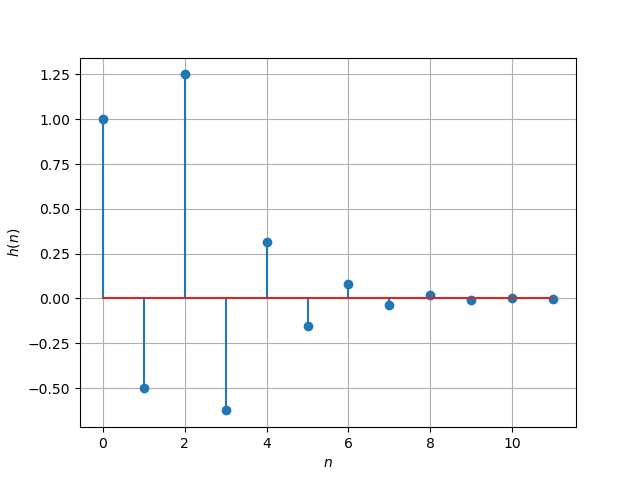
\includegraphics[width=\columnwidth]{figs/5.2.png}
\caption{Plot of $h(n)$}
\label{fig:hn}
\end{figure}
From graph, it is visible that $h(n)$ is bounded.

To check for convergence we can use the ratio test:
\begin{align}
    \lim_{n \to \infty}\abs{\frac{h(n + 1)}{h(n)}} &= \abs{\frac{\brak{-\frac{1}{2}}^{n+1} + \brak{-\frac{1}{2}}^{n-1}}{\brak{-\frac{1}{2}}^{n} + \brak{-\frac{1}{2}}^{n-2}}}\\
    &= \frac{1}{2} < 1 \label{eq:5.5}
\end{align}
Hence, $h(n)$ is convergent.

\item The system with $h(n)$ is defined to be stable if
\begin{equation}
\sum_{n=-\infty}^{\infty}h(n) < \infty \label{eq:5.6}
\end{equation}
Is the system defined by \eqref{eq:iir_filter} stable for the impulse response in \eqref{eq:impulse_resp}?

\solution Sum of infinite terms of a convergent series is finite. From \eqref{eq:5.5}, we proved that $h(n)$ was convergent therefore
\begin{equation}
\sum_{n=-\infty}^{\infty}h(n) < \infty
\end{equation}
Hence, the system with the impulse response $h(n)$ is a stable system.

\item 
Compute and sketch $h(n)$ using 
\begin{equation}
\label{eq:iir_filter_h}
h(n) + \frac{1}{2}h(n-1) = \delta(n) + \delta(n-2), 
\end{equation}
%
This is the definition of $h(n)$.
\\
\solution The following code plots Fig. \ref{fig:hndef}. Note that this is the same as Fig. 
\ref{fig:hn}. 
%
\begin{lstlisting}
wget https://github.com/aroshishp/EE1205/blob/main/Audio_Filtering/codes/5.4.c

wget https://github.com/aroshishp/EE1205/blob/main/Audio_Filtering/codes/5.4.py
\end{lstlisting}
\begin{figure}[!ht]
\centering
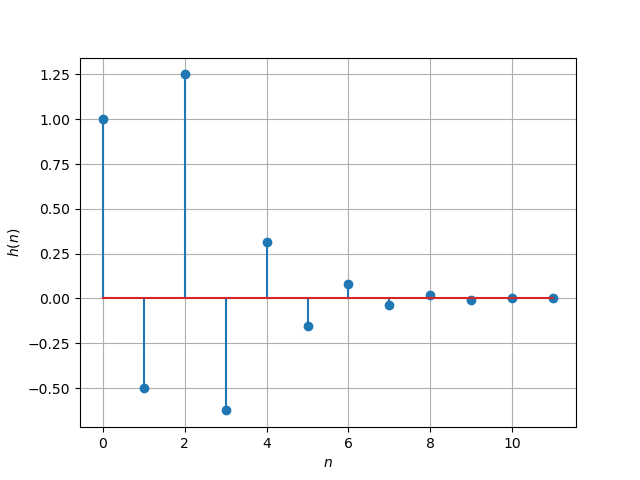
\includegraphics[width=\columnwidth]{figs/5.4.png}
\caption{Plot of $h(n)$ using definition}
\label{fig:hndef}
\end{figure}
%
\item Compute 
%
\begin{equation}
\label{eq:convolution}
y(n) = x(n)*h(n) = \sum_{k=-\infty}^{\infty}x(k)h(n-k) 
\end{equation} 
%
Comment. The operation in \eqref{eq:convolution} is known as
{\em convolution}.
%
\\
\solution The following codes plot Fig. \ref{fig:ynconv}. Note that this is the same as 
$y(n)$ in  Fig. 
\ref{fig:y_n}. 
%
\begin{lstlisting}
wget https://github.com/aroshishp/EE1205/blob/main/Audio_Filtering/codes/5.5.c

wget https://github.com/aroshishp/EE1205/blob/main/Audio_Filtering/codes/5.5.py
\end{lstlisting}
\begin{figure}[!ht]
\centering
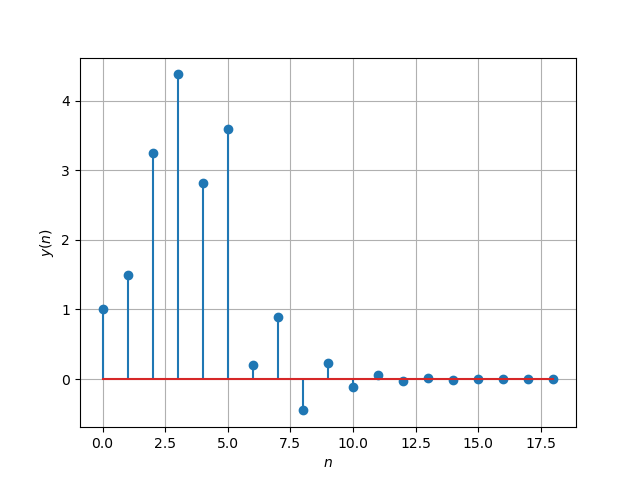
\includegraphics[width=\columnwidth]{figs/5.5.png}
\caption{$y(n)$ using convolution}
\label{fig:ynconv}
\end{figure}
\newpage
\item Show that
\begin{equation}
y(n) =  \sum_{k=-\infty}^{\infty}x(n-k)h(k)
\end{equation}

\solution From \eqref{eq:convolution},
\begin{align}
    y\brak{n} &= \sum_{k=-\infty}^{\infty}x\brak{k}h\brak{n - k}
\end{align}
Substitute $k \to n-k$
\begin{align}
    &= \sum_{n - k=-\infty}^{\infty}x\brak{n - k}h\brak{k} \\
    &= \sum_{k=-\infty}^{\infty}x\brak{n - k}h\brak{k}\label{eq:5.13}
\end{align}
as flipping limits does not change sum.\\

The following codes plot Fig. \ref{fig:5.6}. Note that this is the same as 
$y(n)$ in  Fig. 
\ref{fig:ynconv}.
\begin{lstlisting}
wget https://github.com/aroshishp/EE1205/blob/main/Audio_Filtering/codes/5.6.c

wget https://github.com/aroshishp/EE1205/blob/main/Audio_Filtering/codes/5.6.py
\end{lstlisting}
\begin{figure}[!h]
    \centering
    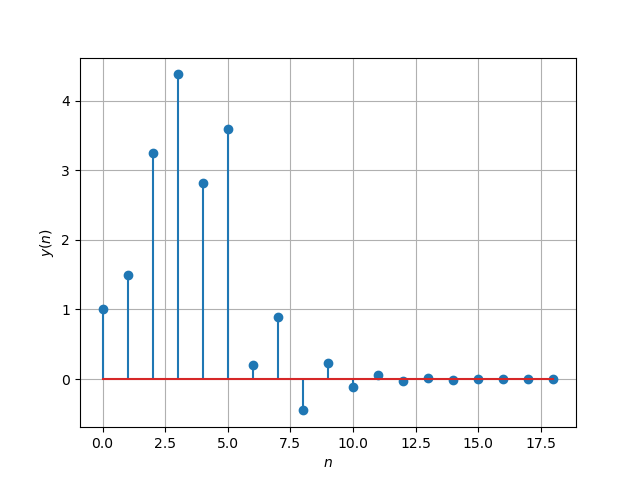
\includegraphics[width = \columnwidth]{figs/5.6.png}
    \caption{Plot of $y(n)$ using \eqref{eq:5.13}}
    \label{fig:5.6}
\end{figure}
\end{enumerate}
\newpage
\section{DFT and FFT}
\begin{enumerate}[label=\thesection.\arabic*]
\item
Compute
\begin{equation}
X(k) \define \sum _{n=0}^{N-1}x(n) e^{-j2\pi kn/N}, \quad k = 0,1,\dots, N-1
\end{equation}
and $H(k)$ using $h(n)$.
\item Compute 
\begin{equation}
Y(k) = X(k)H(k) \label{eq:6.2}
\end{equation}
\item Compute
\begin{equation}
 y\brak{n}={\frac {1}{N}}\sum _{k=0}^{N-1}Y\brak{k}\cdot e^{j 2\pi kn/N},\quad n = 0,1,\dots, N-1
\end{equation}
\\
\solution The following code plots Fig. \ref{fig:yndft} by taking {\em Inverse Discrete Fourier Transform} (IDFT) of $Y(k)$. Note that this is also the same as 
$y(n)$ in  Fig. 
\ref{fig:y_n}. It also prints out the values of $X(k)$, $H(k)$, $Y(k)$, and $y(n)$.
%
\begin{lstlisting}
wget https://github.com/aroshishp/EE1205/blob/main/Audio_Filtering/codes/6.123.py
\end{lstlisting}
\begin{figure}[!ht]
\centering
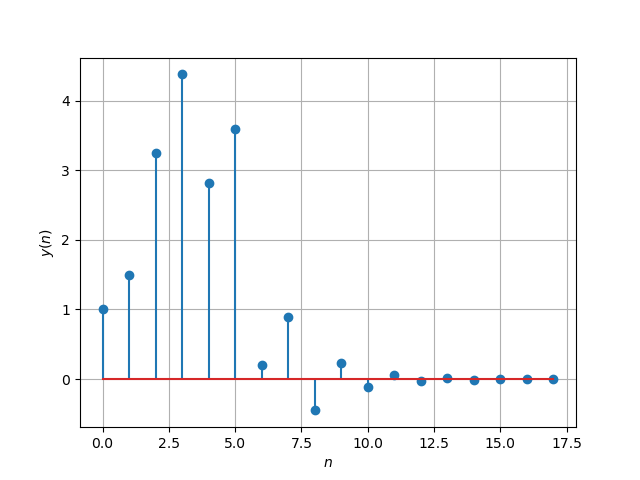
\includegraphics[width=\columnwidth]{figs/6.1.png}
\caption{$y(n)$ from IDFT}
\label{fig:yndft}
\end{figure}
\newpage
\item Repeat the previous exercise by computing $X(k), H(k)$ and $y(n)$ through FFT and 
IFFT.\\

\solution The code below calculates $X(k)$, $H(k)$ using FFT and plots the graph of $y(n)$ using IFFT and IDFT both (to compare).
\begin{lstlisting}
wget https://github.com/aroshishp/EE1205/blob/main/Audio_Filtering/codes/6.4.py
\end{lstlisting}
\begin{figure}[!h]
    \centering
    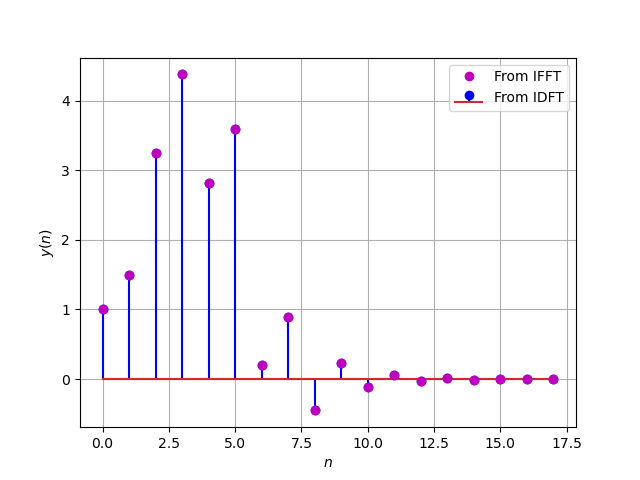
\includegraphics[width = \columnwidth]{figs/6.4.png}
    \caption{Plot of $y(n)$ from IDFT and IFFT}
    \label{fig:enter-label}
\end{figure}

\item Wherever possible, express all the above equations as matrix equations.
\\

\solution The DFT matrix is given by: 
\begin{align}
	\mtx{W} = 
	\begin{pmatrix}
		\omega^0 & \omega^0 & \ldots & \omega^0 \\
		\omega^0 & \omega^1 & \ldots & \omega^{N - 1} \\
		\vdots & \vdots & \ddots & \vdots \\
		\omega^0 & \omega^{N - 1} & \ldots & \omega^{(N -1)(N - 1)}
	\end{pmatrix}
\end{align}
where $\omega=e^{-\frac{j2\pi}{N}}$ . General DFT equation is given by:
\begin{align}
    \mtx{X} = \mtx{W}\mtx{x}
\end{align}
where
\begin{align}
	\mtx{x} = 
	\begin{pmatrix}
		x(0) \\ x(1) \\ \vdots \\ x(n - 1)
	\end{pmatrix}
\end{align}
\begin{align}
	\mtx{X} = 
	\begin{pmatrix}
		X(0) \\ X(1) \\ \vdots \\ X(n - 1)
	\end{pmatrix}
\end{align}
Then from \eqref{eq:6.2}:
\begin{align}
	\mtx{Y} = \mtx{X}\odot\mtx{H} = \brak{\mtx{W}\mtx{x}}\odot\brak{\mtx{W}\mtx{h}}
\end{align}
where $\odot$ represents the Hadamard product which multiplies corresponding elements of matrices of same size.

The below code computes $y\brak{n}$ by DFT Matrix and then plots it.
\begin{lstlisting}
wget https://github.com/aroshishp/EE1205/blob/main/Audio_Filtering/codes/6.5.py
\end{lstlisting}
\begin{figure}[!h]
    \centering
    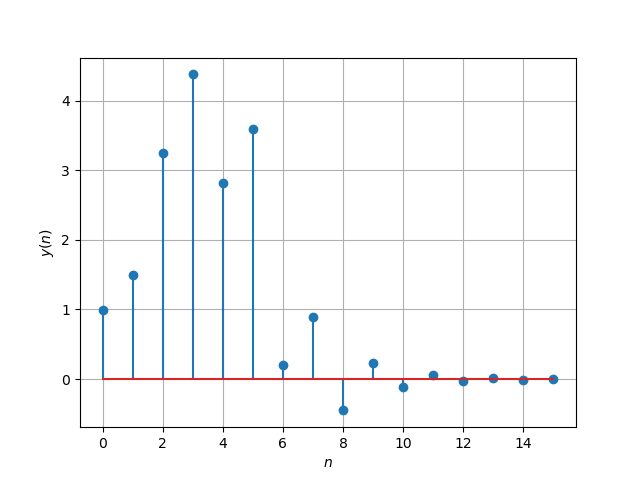
\includegraphics[width = \columnwidth]{figs/6.5.png}
    \caption{Plot of $y(n)$ using matrix method}
    \label{fig:enter-la}
\end{figure}
\end{enumerate}
\section{Exercises}

Answer the following questions by looking at the python code in Problem \ref{prob:output}.
\begin{enumerate}[label=\thesection.\arabic*]
\item
The command
\begin{lstlisting}
output_signal = signal.lfilter(b, a, input_signal)
	\end{lstlisting}
in Problem \ref{prob:output} is executed through the following difference equation
\begin{equation}
\label{eq:iir_filter_gen}
 \sum _{m=0}^{M}a\brak{m}y\brak{n-m}=\sum _{k=0}^{N}b\brak{k}x\brak{n-k}
\end{equation}
%
where the input signal is $x(n)$ and the output signal is $y(n)$ with initial values all 0. Replace
\textbf{signal.filtfilt} with your own routine and verify.
\\

\solution The code below plots the output of scipy.signal.lfilter and the output of custom function on the same graph.
\begin{lstlisting}
wget https://github.com/aroshishp/EE1205/blob/main/Audio_Filtering/codes/lfilter.py
\end{lstlisting}
\begin{figure}[!h]
    \centering
    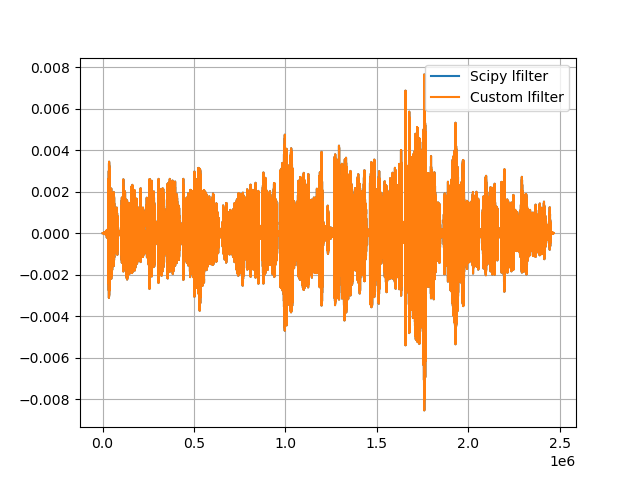
\includegraphics[width = \columnwidth]{figs/lfilter.png}
    \caption{Output of signal.lfilter and custom routine}
    \label{fig:7.1}
\end{figure}
Both the plots overlap, indicating that the custom filter code does the same function as scipy.signal.lfilter.
\item Repeat all the exercises in the previous sections for the above $a$ and $b$.\\

\solution The code in \ref{py:filter} calculates values of a and b and prints them:
$
\begin{array}{c}
  a = [ 1.000         \quad -1.792 \quad 1.518 \quad -0.608 \quad 0.098] \\
b = [0.013\quad 0.054 \quad 0.081\quad 0.054 \quad 0.013]
\end{array}
$
Now, using \eqref{eq:iir_filter_gen}, difference equation:
\begin{multline}
a\brak{0}y\brak{n} + a\brak{1}y\brak{n-1}+a\brak{2}y\brak{n-2}\\
+a\brak{3}y\brak{n-3}+a\brak{4}y\brak{n-4} =   b\brak{0}x\brak{n} \\
+ b\brak{1}x\brak{n-1}+b\brak{2}x\brak{n-2}+b\brak{3}x\brak{n-3}\\
+b\brak{4}x\brak{n-4} 
\end{multline}
Substituting,
\begin{multline}
    y\brak{n} -1.792y\brak{n-1}+1.518y\brak{n-2}\\
-0.608y\brak{n-3}+0.098y\brak{n-4} = 0.013x\brak{n} \\
+ 0.054x\brak{n-1}+0.081x\brak{n-2}+0.054x\brak{n-3}\\
+0.013x\brak{n-4} 
\end{multline}
The rational transfer function describing this filter in the z-transform domain is:
\begin{align}
     H(z) &= \frac{b(0) + b(1) z^{-1} + b(2) z^{-2} + \ldots + b(N) z^{-N}}{a(0) + a(1) z^{-1} + a(2) z^{-2} + \ldots + a(M) z^{-M}}\\ \label{eq:7.4}
    &= \frac{\sum_{k = 0}^{N}b(k)z^{-k}}{\sum_{k = 0}^{M}a(k)z^{-k}}
\end{align}
In our case, $M=N=4$.

Now, the partial fraction of \eqref{eq:7.4} is given by:
\begin{align}
   H\brak{z}&= \sum_{i}\frac{r(i)}{1 - p(i)z^{-1}} + \sum_{j}k(j)z^{-j}\label{eq:7.6}
\end{align}
Values of $r(i)$, $p(i)$ and $k(j)$ are calculated using scipy.signal.residuez, which returns the above mentioned series:
\begin{table}[!h]
    \centering
    \renewcommand\thetable{1}
    \resizebox{0.51\textwidth}{!}{
    \begin{tabular}{|c|c|c|}
    \hline
    \textbf{$r\brak{i}$} & \textbf{$p\brak{i}$} & \textbf{$k\brak{i}$} \\ \hline
    $0.28018185-1.23886252j$ &$0.38674749+0.17013423j$&$0.13702919$  \\ \hline
    $0.28018185+1.23886252j$ &$0.38674749-0.17013423j$&$-$  \\ \hline
    $-0.3419458 +0.19576406j$ &$0.50928445+0.54087922j$&$-$  \\ \hline
    $-0.3419458 -0.19576406j$ &$0.50928445-0.54087922j$&$-$  \\ \hline
    \end{tabular}}
    \caption{Values of $r(i)$, $p(i)$, $k(i)$}
    \label{tab:residuez}
\end{table}


Inverse of \eqref{eq:7.6} is given using:
\begin{align}
    a^{n}u\brak{n} &\system \frac{1}{1-az^{-1}}\\
    \delta\brak{n-k} &\system z^{-k}\\
    \implies h(n) &= \sum_{i}r(i)[p(i)]^nu(n) + \sum_{j}k(j)\delta(n - j)
\end{align}
Code to plot $h(n)$:
\begin{lstlisting}
wget https://github.com/aroshishp/EE1205/blob/main/Audio_Filtering/codes/7.2hn.py
\end{lstlisting}

\textbf{Plot of h(n)}:
\begin{figure}[!h]
    \centering
    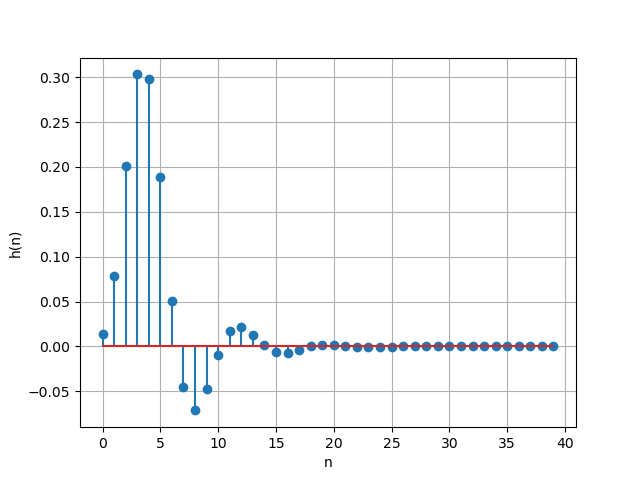
\includegraphics[width = \columnwidth]{figs/7.2hn.png}
    \caption{Plot of $h(n)$}
    \label{fig:7.2}
\end{figure}

Code to plot Pole-Zero Plot:
\begin{lstlisting}
wget https://github.com/aroshishp/EE1205/blob/main/Audio_Filtering/codes/7.2pole.py
\end{lstlisting}
\begin{figure}[!h]
    \centering
    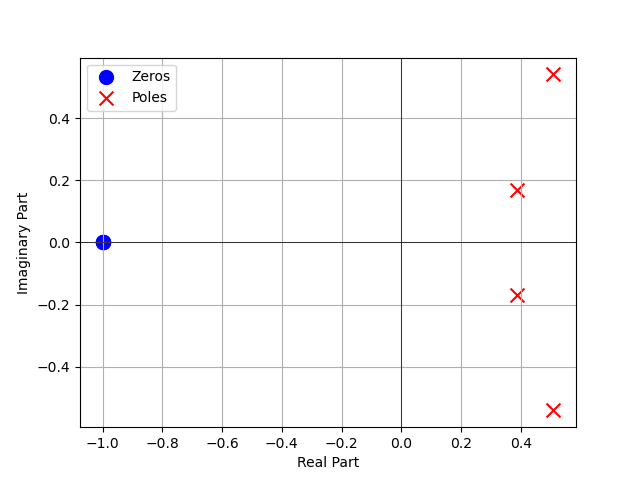
\includegraphics[width = \columnwidth]{figs/7.2zp.png}
    \caption{Pole-Zero Plot}
    \label{fig:7.2zp}
\end{figure}
There are complex poles, so $h(n)$ has a damped sinusoidal form.\\

\textbf{Stability of System}
\begin{align}
H\brak{z} &= \sum_{n = 0}^{\infty} h\brak{n}z^{-n}\\
\implies H(1)&= \sum_{n = 0}^{\infty}h(n) \\
&= \frac{\sum_{k = 0}^{N}b(k)}{\sum_{k = 0}^{M}a(k)}< \infty
\end{align}
as both $a\brak{k}$ and $b\brak{k}$ are finite length sequences.\\
Then, \eqref{eq:5.6} implies $h(n)$ is impulse response of a stable system.
\\
Code to plot Frequency Response:
\begin{lstlisting}
wget https://github.com/aroshishp/EE1205/blob/main/Audio_Filtering/codes/7.2hw.py
\end{lstlisting}

\textbf{Frequency Response of Butterworth Filter}
\begin{figure}[!h]
    \centering
    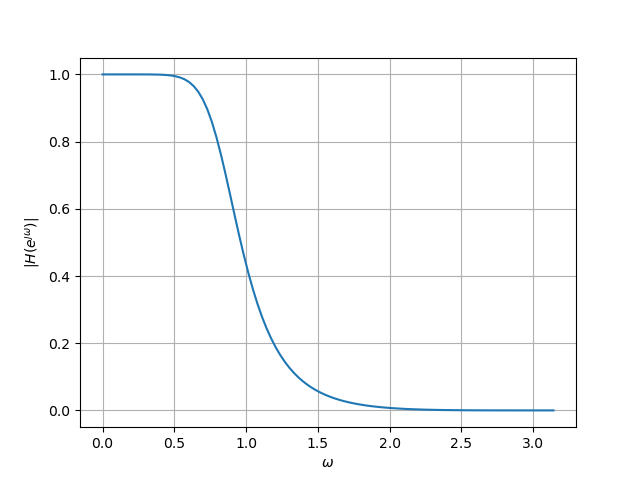
\includegraphics[width = \columnwidth]{figs/7.2hw.png}
    \caption{Plot of Frequency Response}
    \label{fig:7.2hw}
\end{figure}
\\
\textbf{Frequency Response of Butterworth Filter in Analog Domain}

To convert to analog domain, we can use the Bilinear Transform where we substitute:
\begin{align}
    z=\frac{1+\frac{sT}{2}}{{1-\frac{sT}{2}}}
\end{align}
Code to plot Frequency Response in Analog Domain:
\begin{lstlisting}
wget https://github.com/aroshishp/EE1205/blob/main/Audio_Filtering/codes/7.2bt.py
\end{lstlisting}
\begin{figure}[!h]
    \centering
    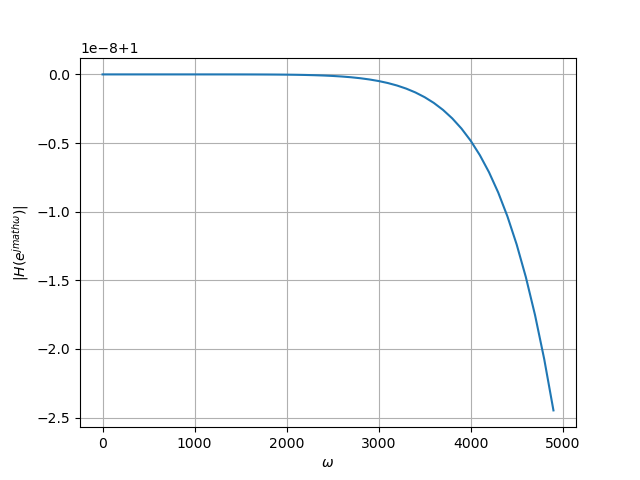
\includegraphics[width = \columnwidth]{figs/7.2bt.png}
    \caption{Plot of Frequency Response in Analog Domain}
    \label{fig:7.2bt}
\end{figure}

\textbf{Convolution}\\
We calculate
\begin{equation}
    y(n) = x(n)*h(n) = \sum_{k=-\infty}^{\infty}x(k)h(n-k) 
\end{equation}

through the following code. The code plots input signal $x(n)$ and output $y(n)$ obtained from lfilter and through convolution.
\begin{lstlisting}
wget https://github.com/aroshishp/EE1205/blob/main/Audio_Filtering/codes/7.2conv.py
\end{lstlisting}
\begin{figure}[!h]
    \centering
    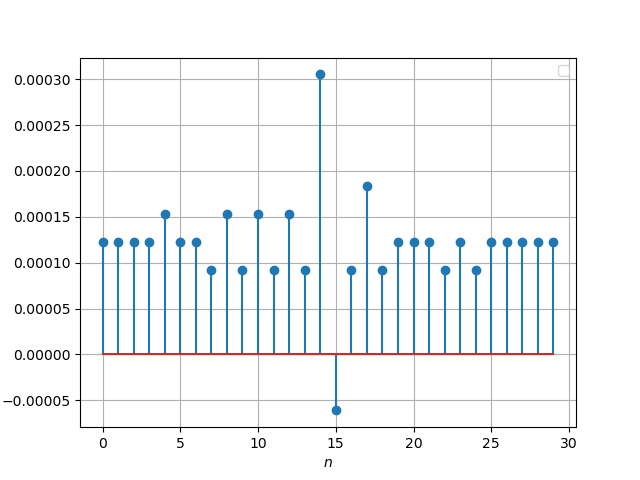
\includegraphics[width = \columnwidth]{figs/input.png}
    \caption{Plot of Input Signal $x(n)$}
    \label{fig:input}
\end{figure}
\begin{figure}[!h]
    \centering
    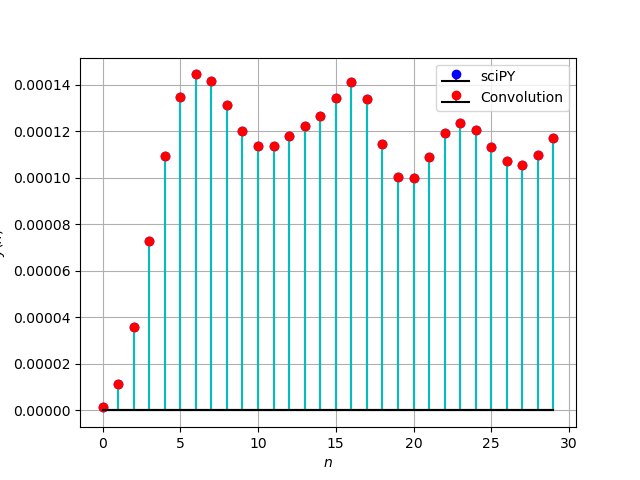
\includegraphics[width = \columnwidth]{figs/output.png}
    \caption{Plot of Output Signal $y(n)$ from lfilter and convolution}
    \label{fig:output}
\end{figure}
\newpage
\textbf{DFT and FFT}\\
Code to calculate DFT/IDFT and FFT/IFFT are written below. $y(n)$ is plotted from lfilter output, DFT/IDFT and FFT/IFFT on the same graph and they overlap.
\begin{lstlisting}
wget https://github.com/aroshishp/EE1205/blob/main/Audio_Filtering/codes/7.2dft.py
\end{lstlisting}
\begin{figure}[!h]
    \centering
    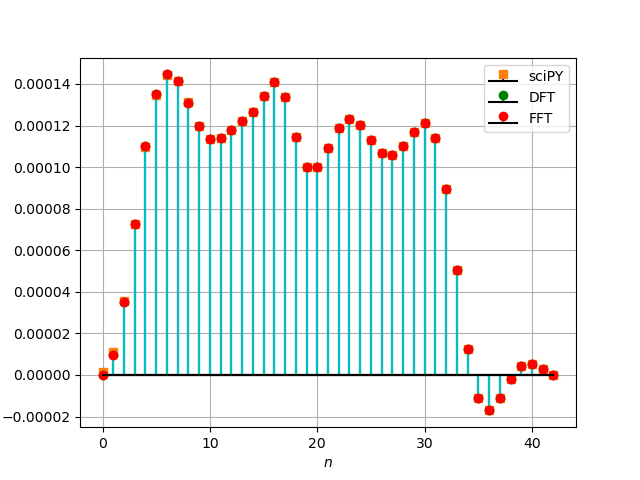
\includegraphics[width = \columnwidth]{figs/7.2dft.png}
    \caption{Plot of Output Signal from above mentioned methods}
    \label{fig:output_dft}
\end{figure}
\item Implement your own FFT routine in C and call this FFT in python
\\
\solution The below C code implements the FFT algorithm:
\begin{lstlisting}
wget https://github.com/aroshishp/EE1205/blob/main/Audio_Filtering/codes/7.3.c
\end{lstlisting}
Run the following command to generate a shared library '7.3.so':
\begin{lstlisting}
gcc -shared -o 7.3.so -fPIC 7.3.c
\end{lstlisting}
The C code is called in the following Python code and output is printed. It can be seen that the same output is printed through both codes.
\begin{lstlisting}
wget https://github.com/aroshishp/EE1205/blob/main/Audio_Filtering/codes/7.3.py
\end{lstlisting}

\item Find the Time Complexities of computing $y(n)$ using FFT/IFFT and convolution and compare. 
\\
\solution The below codes generate and plot the time complexities of computing $y(n)$ using FFT/IFFT and Convolution:
\begin{lstlisting}
wget https://github.com/aroshishp/EE1205/blob/main/Audio_Filtering/codes/7.4.c

wget https://github.com/aroshishp/EE1205/blob/main/Audio_Filtering/codes/7.4.py
\end{lstlisting}
\begin{figure}[!h]
    \centering
    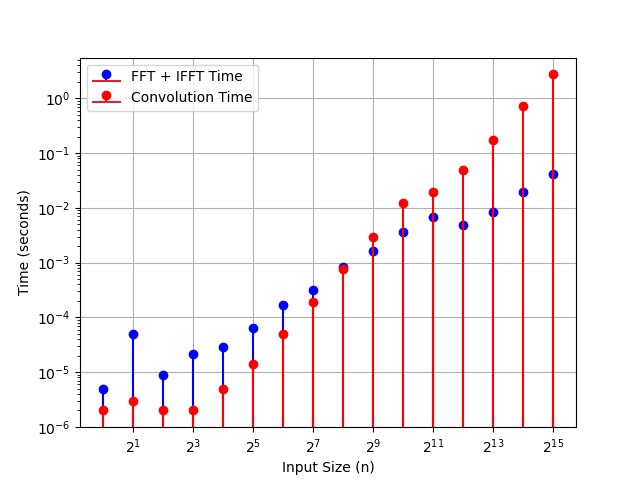
\includegraphics[width = \columnwidth]{figs/7.4.png}
    \caption{Comparison of Time Complexities}
    \label{fig:7.4}
\end{figure}
Time complexity of FFT/IFFT method is $O(n\log(n))$ and that of Convolution method is $O(n^2)$.
\\
\item What is the sampling frequency of the input signal?
\\
\solution
Sampling frequency (fs) = $44100$ Hz. It can be printed from \ref{py:filter}.
\\
\item
What is type, order and  cutoff-frequency of the above butterworth filter
\\
\solution
The given Butterworth Filter is low pass with order=4 and cutoff-frequency = 6kHz.
\\
\item
Modifying the code with different input parameters and to get the best possible output.
\\
\solution The best filtered audio output was obtained by setting order to 4 and keeping cutoff frequency at 6000 Hz. These parameters were used for the spectrogram output as well as for this section.
\end{enumerate}

\end{document}
